\documentclass[titlepage,landscape]{seminar}
\usepackage{url}
\usepackage{graphicx}
\usepackage[pdftex]{color}
\usepackage{hyperref}
\usepackage{epstopdf}
\usepackage{slides}

\newcommand{\frack}{\frac{1}{k}}

\begin{document}

\myslide{
\[
Var(p_{t+1}) = \frac{p_t(1-p_t)}{2N} \quad.
\]
\vfil
\[
N_e^{(v)} = \frac{p(1-p)}{2\widehat{Var}(p)}
\]
}

\myslide{
\[
f_{t+1}
   = \frac{1}{2N} + \left(1 - \frac{1}{2N}\right)f_t
\]
\vfil
\[
N_e^{(f)} = \frac{1 - \hat f_t}{2(\hat f_{t+1} - \hat f_t)}
\]
\vfil
Assume $\hat f_t = 0$
\[
N_e^{(f)} = \frac{1}{2\hat f_{t+1}}
\]
}

\myslide{
\[
f_{t+1} = \left(\left(\frac{1}{2N}\right) +
          \left(1 - \frac{1}{2N}\right)f_t\right)(1-\mu)^2
\]
}

\myslide{
\begin{eqnarray*}
\hat f &=& \left(\left(\frac{1}{2N}\right) +
          \left(1 - \frac{1}{2N}\right)\hat f\right)(1-\mu)^2 \\
\hat f\left(1 - 
\left(1 - \frac{1}{2N}\right)(1-\mu)^2\right)
       &=& \left(\frac{1}{2N}\right)(1-\mu)^2 \\
\hat f &=& \frac{\left(\frac{1}{2N}\right)(1-\mu)^2}
           {1 -\left(1 - \frac{1}{2N}\right)(1-\mu)^2} \\
       &\approx& \frac{1 - 2\mu}
           {2N\left(1 - \left(1 - \frac{1}{2N}\right)(1-2\mu)\right)} \\
       &=& \frac{1 - 2\mu} 
           {2N\left(1 - 1 + \frac{1}{2N} + 2\mu -
            \frac{2\mu}{2N}\right)} \\
       &=& \frac{1 - 2\mu}{1 + 4N\mu - 2\mu} \\
       &\approx& \frac{1}{4N\mu + 1}
\end{eqnarray*}
}

\myslide{
\begin{center}
\resizebox{!}{7.5cm}{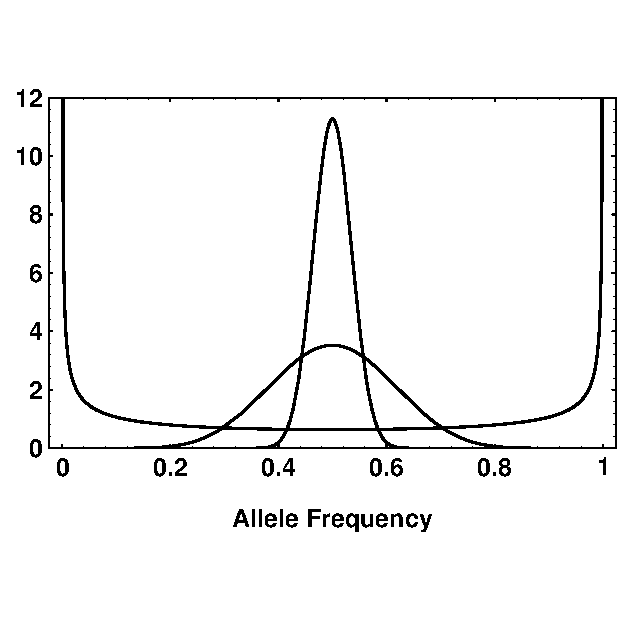
\includegraphics{mutation.eps}}
\end{center}
}

\myslide{
\[
f_{t+1} = \left(\left(\frac{1}{2N}\right) +
          \left(1 - \frac{1}{2N}\right)f_t\right)(1-m)^2
\]
\vfill
\[
\hat f \approx \frac{1}{4Nm + 1}
\]
}

\myslide{
\begin{center}
\begin{tabular}{ccc}
\hline\hline
$A_1A_1$ & $A_1A_2$      & $A_2A_2$ \\
\hline
1 + s    & $1 + \half s$ & 1 \\
\hline
\end{tabular}
\end{center}
\vfill
\[
P_1(p) = \frac{1 - e^{-2N_esp}}{1 - e^{-2N_es}}
\]
}

\myslide{
\[
P_1(p) = \frac{1 - e^{-2N_esp}}{1 - e^{-2N_es}}
\]
\vfill
\begin{eqnarray*}
P_1(p) &=& \frac{1 - e^{-2N_es(1/2N)}}{1 - e^{-2N_es}} \\
       &\approx& 1 - e^{-N_es(1/N)} \hbox{ if $2N_es$ is ``large''} \\
       &\approx& s\left(\frac{N_e}{N}\right)
                 \hbox{ if $s$ is ``small.''}
\end{eqnarray*}
}

\myslide{
\begin{table}
\begin{center}
\begin{tabular}{l|cc}
\hline\hline
      & \multicolumn{2}{c}{$N_e$} \\
$s$   & 4                  & 100 \\
\hline
0.001 & $1 \times 10^{-2}$ & $9 \times 10^{-3}$ \\
0.01  & $1 \times 10^{-2}$ & $3 \times 10^{-3}$ \\
0.1   & $7 \times 10^{-3}$ & $5 \times 10^{-10}$ \\
\hline
\end{tabular}
\end{center}
\caption{Fixation probabilities for a deleterious mutation as a
function of effective population size and selection coefficient for a
newly arisen mutant ($p=0.01$).}
\end{table}
}

\myslide{
\begin{center}
\resizebox{!}{5cm}{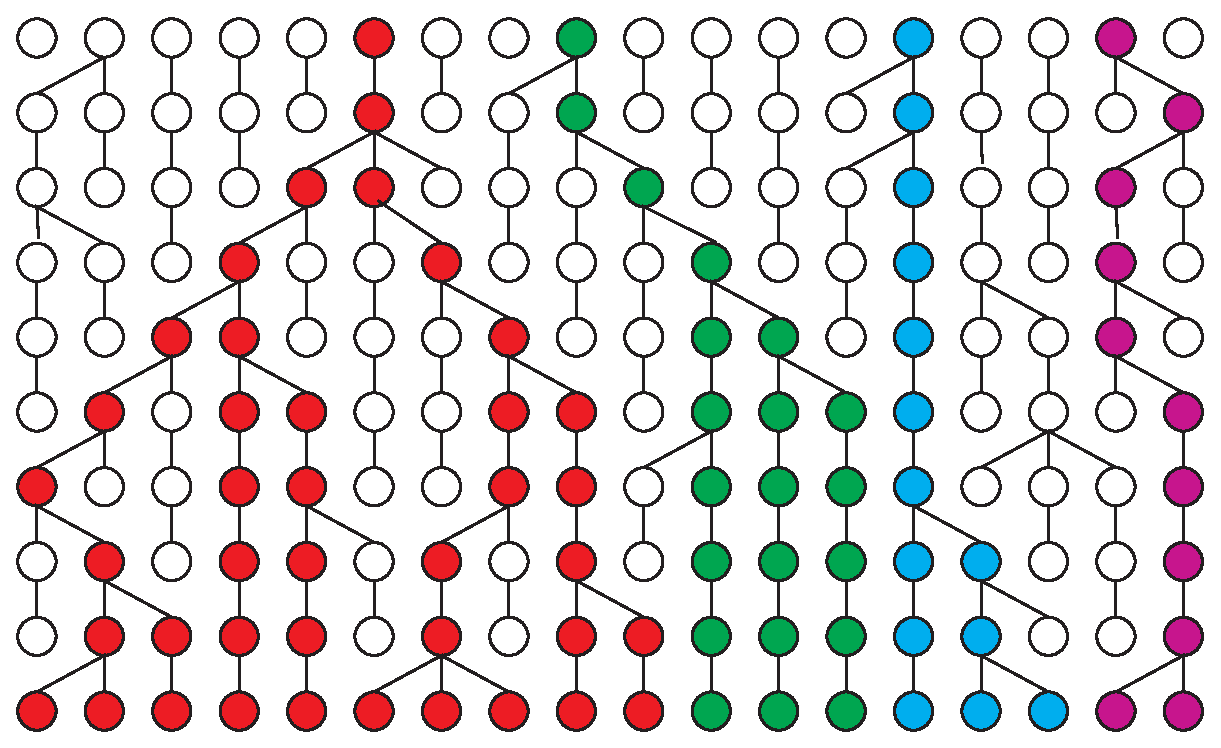
\includegraphics{coalescent-figure.eps}}
\end{center}
}

\myslide{
Probability of coalescent event in last generation
\[
\frac{1}{2N_e^{(f)}}
\]
Probability of no coalescent event in last generation
\[
1 - \frac{1}{2N_e}
\]
}

\myslide{
Probability of coalescent event in last generation
\[
\frac{1}{2N_e^{(f)}}
\]
Probability of no coalescent event in last generation
\[
1 - \frac{1}{2N_e}
\]
Probability of coalescent event $t$ generations ago
\[
\left(1 -
\frac{1}{2N_e}\right)^{t-1}\left(\frac{1}{2N_e}\right)
\]
}

\myslide{
Probability of coalescent event in last generation
\[
\left(\frac{1}{2N_e}\right)\left(\frac{m(m-1)}{2}\right)
\]
Probability of coalescent event $t$ generations ago
\[
\left(1-\left(\frac{1}{2N_e}\right)\left(\frac{m(m-1)}{2}\right)\right)^{t-1}
\left(\frac{1}{2N_e}\right)\left(\frac{m(m-1)}{2}\right)
\]
\vfill
Time to coalescence of all alleles approximately $4N_e$ generations
}

\myslide{
Coalescent times in a structured population
\begin{eqnarray*}
\bar t_0 &=& \mbox{mean coalescence time within populations} \\
\bar t &=& \mbox{mean coalescence time of randomly chosen alleles}
\end{eqnarray*}
\vfill
\[
F_{ST} = \frac{\bar t - \bar t_0}{\bar t}
\]

}

\end{document}

